\chapter{Языковые средства формального описания синтаксиса и денотационной семантики естественных языков в ostis-системах}
\chapauthortoc{Никифоров С.А.\\Гойло А.А.}
\label{chapter_lang}

\vspace{-7\baselineskip}

\begin{SCn}
    \begin{scnrelfromlist}{автор}
        \scnitem{Никифоров С.А.}
        \scnitem{Гойло А.А.}
    \end{scnrelfromlist}

    \bigskip

    \scntext{аннотация}{Глава посвящена языковым средствам формального описания \textit{синтаксиса} и \textit{денотационной семантики} различных \textit{языков} в \textit{ostis-системах}. Предложена \textit{онтология} различных \textit{языков}. Формализованы базовые \textit{синтаксические правила} построения конструкций \textit{естественных языков} и \textit{правила соответствия синтаксических конструкций семантическому представлению}.}

    \bigskip

    \begin{scnrelfromlist}{подраздел}
        \scnitem{\ref{section_natural_language_syntax_formalization}~\nameref{section_natural_language_syntax_formalization}}
        \scnitem{\ref{section_natural_language_denotational_semantics_formalization}~\nameref{section_natural_language_denotational_semantics_formalization}}
    \end{scnrelfromlist}

    \bigskip

    \begin{scnrelfromlist}{ключевое понятие}
        \scnitem{язык}
        \scnitem{лексема}
        \scnitem{грамматическая категория}
        \scnitem{часть речи}
        \scnitem{словоформа}
        \scnitem{составляющая}
        \scnitem{синтаксическая группа}
        \scnitem{вершина}
        \scnitem{комплемент}
        \scnitem{адъюнкт}
        \scnitem{спецификатор}
    \end{scnrelfromlist}

    \begin{scnrelfromlist}{ключевое знание}
        \scnitem{Общие правила синтаксической структуры конструкций естественных языков}
        \scnitem{Правила построения синтаксических групп}
        \scnitem{Базовые правила денотационной семантики естественных языков}
    \end{scnrelfromlist}

    \bigskip

    \begin{scnrelfromlist}{библиографическая ссылка}
        \scnitem{\scncite{Golenkov2021}}
        \scnitem{\scncite{Pileggi2018}}
        \scnitem{\scncite{Lando2007}}
        \scnitem{\scncite{Farrar2002}}
        \scnitem{\scncite{Chiarcos2012}}
        \scnitem{\scncite{Text2022}}
        \scnitem{\scncite{EAGLES2022}}
        \scnitem{\scncite{Ide2010}}
        \scnitem{\scncite{Schalley2019}}
        \scnitem{\scncite{Mccrae2015}}
        \scnitem{\scncite{GOLD2022}}
        \scnitem{\scncite{Pease2002}}
        \scnitem{\scncite{Farrar2003}}
        \scnitem{\scncite{Chiarcos2012a}}
        \scnitem{\scncite{Bateman1997}}
        \scnitem{\scncite{Bateman2002}}
        \scnitem{\scncite{Buitelaar2009}}
        \scnitem{\scncite{Kostareva2016}}
        \scnitem{\scncite{Nevzorova2019}}
        \scnitem{\scncite{Cimiano2013}}
        \scnitem{\scncite{Bouayad2014}}
        \scnitem{\scncite{Saha2016}}
        \scnitem{\scncite{Shamsfard2004}}
        \scnitem{\scncite{Bateman2010}}
        \scnitem{\scncite{Moens1987}}
        \scnitem{\scncite{Dobrov2018}}
        \scnitem{\scncite{WordNet}}
        \scnitem{\scncite{VerbNet}}
        \scnitem{\scncite{FrameNet}}
        \scnitem{\scncite{Pease2010}}
        \scnitem{\scncite{Matsukawa1991}}
        \scnitem{\scncite{Calzolari1991}}
        \scnitem{\scncite{Buitelaar2006a}}
        \scnitem{\scncite{Buitelaar2006b}}
        \scnitem{\scncite{Cimiano2007}}
        \scnitem{\scncite{McCrae2012}}
        \scnitem{\scncite{SemanticWeb}}
        \scnitem{\scncite{NLTK}}
        \scnitem{\scncite{Spacy}}
        \scnitem{\scncite{Erekhinskaya2020}}
        \scnitem{\scncite{Standart2021}}
        \scnitem{\scncite{SILGlossary}}
        \scnitem{\scncite{Adger2003}}
        \scnitem{\scncite{Jackendoff1977}}
        \scnitem{\scncite{Haegeman1994}}
        \scnitem{\scncite{Carnie2012}}
        \scnitem{\scncite{Heim1998}}
        \scnitem{\scncite{Winter2016}}
        \scnitem{\scncite{Portner2008}}
    \end{scnrelfromlist}

\end{SCn}

\section*{Введение в Главу~\ref{chapter_lang}}

В настоящее время научные исследования в области искусственного интеллекта развиваются по большому спектру различных направлений, однако между ними отсутствует согласованность систем понятий и, как следствие этого, совместимость разрабатываемых систем (см.~\scncite{Golenkov2021}).

Так в области создания программного обеспечения в силу его значительной сложности остро стоит проблема обеспечения интероперабельности различных программных сущностей, а также переиспользования результатов предыдущих аналогичных разработок.

Одним из путей решения данных проблем является создание \textit{онтологий} программного обеспечения (см.~\textit{\ref{sec_ontology}~\nameref{sec_ontology}}, \textit{\ref{sec_programs_ontologies}~\nameref{sec_programs_ontologies}}), к которым предъявляются следующие требования (см.~\scncite{Pileggi2018}):
\begin{textitemize}
    \item путем спецификация формальной семантики для избежания двусмысленных определений, а также нежелательных интерпретаций с целью обеспечения интероперабельности;
    \item созданные \textit{онтологии} должны быть применены в иной или же более широкой предметной области, что позволило бы избежать дорогостоящей специальной разработки и может повысить качество конечного продукта;
    \item возможность применения на их базе механизмов логического вывода.
\end{textitemize}

В качестве примера \textit{онтологии} в данной области можно привести COPS (см.~\scncite{Lando2007}).
Целью данной \textit{онтологии} являлась формализация общих понятий из области программного обеспечения с целью упрощения его разработки и использования.

Проблема совместимости результатов исследований также остро стоит и в лингвистике --- науке, в которой существует множество различных теорий, часто несовместимых друг с другом.
В лингвистических исследованиях используются разные варианты разметки данных, нет одного подхода к структуризации корпусов текстов и различаются способы представления данных в них (см.~\scncite{Farrar2002},~\scncite{Chiarcos2012}).

В качестве решения проблемы несовместимости различных способов описания данных в лингвистике предлагались варианты стандартизации форматов такого описания.
Примером могут служить \textit{Text Encoding Initiative} --- консорциум по стандартизации представления текстов в цифровом виде (см.~\scncite{Text2022}) и гайдлайны экспертной группы по стандартизации представления языковых данных \textit{EAGLES} (например, рекомендации по разметке корпусов текстов (см.~\scncite{EAGLES2022}).
Однако ни один из таких стандартов не получил распространения и не стал использоваться лингвистами повсеместно (см.~\scncite{Ide2010} (с.~4))).

Вместо создания рекомендаций по разметке языкового материала в качестве более эффективного средства решения указанных выше проблем предлагается создание \textit{онтологий} (см.~\scncite{Schalley2019},~\scncite{Mccrae2015}).
Помимо того, что \textit{онтология верхнего уровня} для предметной области языкознания может служить связующим звеном между различными лингвистическими теориями, она также представляет собой формализованное описание лингвистических концептов, представленное в удобном для компьютеров формате, что обусловливает ее применимость в системах, способных понимать аннотированные языковые данные, совершать интеллектуальный поиск по корпусам текстов, а также потенциально выполнять анализ существующих лингвистических исследований (см.~\scncite{Farrar2002}).

В качестве такой \textit{онтологии} в предметной области лингвистики выступает \textit{The General Ontology of Linguistic Description} (\textit{GOLD}) (см.~\scncite{GOLD2022}).
В этой \textit{онтологии} формализованы наиболее базовые категории и отношения, используемые в лингвистике, а сама онтология интегрирована с онтологией верхнего уровня \textit{Suggested Upper Merged Ontology} (\textit{SUMO}) (см.~\scncite{Pease2002}).
Авторы \textit{GOLD} пишут, что создавали онтологию в первую очередь для того, чтобы решить проблему интероперабельности данных лингвистической типологии и для того, чтобы с ее помощью экспертные системы могли обрабатывать научные данные по естественным языкам --- то есть целью создателей \textit{онтологии} не являлось непосредственно решение задач из области обработки текстов на естественном языке (см.~\scncite{Farrar2003} (с.4)).

\textit{онтологией} естественных языков, нацеленной непосредственно на использование при решении задач по обработке естественного языка, является \textit{Ontologies of Linguistic Annotation} (\textit{OLiA}) (см.~\scncite{Chiarcos2012a}).
Основной идеей \textit{онтологии} является обеспечение совместимости разметки языковых данных, полученных в результате выполненного компьютерными системами анализа текстов на \textit{естественном языке} с соответствующими им лингвистическими концептами из \textit{онтологии} --- в отличие от других лингвистических \textit{онтологий}, \textit{OLiA} предоставляет не только инвентарь концептов и отношений, но и необходимую спецификацию интеграции этих элементов с разметкой языковых данных (например, в корпусах (см.~\scncite{Chiarcos2012a} (c.~4)).

При создании \textit{онтологий} \textit{естественного языка}, встает вопрос о статусе спецификации лингвистической информации в таких онтологиях.
Дж. Бейтман выделяет три типа онтологий в зависимости от интегрированности в них естественно-языковой информации (см.~\scncite{Bateman1997}):
\begin{textitemize}
    \item \textit{онтологии}, представляющие собой абстрактную семантико-концептуальную репрезентацию знаний о мире, которая используется непосредственно в качестве \textit{денотационной семантики} для \textit{синтаксиса} и \textit{лексики} естественного языка;
    \item \textit{онтологии}, в которых есть отдельная спецификация \textit{денотационной семантики} \textit{естественного языка}, которая служит интерфейсом между \textit{синтаксисом} естественных \textit{языков} и концептуальной онтологией;
    \item \textit{онтологии}, представляющие собой абстрактную спецификацию \textit{знаний} о реальном мире вне зависимости от ограничений \textit{естественного языка}.
\end{textitemize}

Популярность в сфере обработки естественного языка приобрел второй тип \textit{онтологии} (см.~\scncite{Bateman1997} (c.~8)), так как он, в отличие от третьего подхода, который совсем не формализует лингвистическую информацию, позволяет специфицировать больше информации о естественных языках.
Так, одна из самых популярных онтологий, используемых в системах для обработки естественного языка, the \textit{Generalized Upper Model} (см.~\scncite{Bateman2002}), является онтологией второго типа (см.~\scncite{Bateman1997}).
П. Буителар и другие подчеркивают, что всем \textit{формальным онтологиям} необходима связь с языковой информацией для решения таких задач как выделение информации из текстов \textit{естественного языка}, автоматизированное заполнение \textit{онтологий} и генерации текста на \textit{естественном языке} (см.~\scncite{Buitelaar2009}).

Так как использование онтологий в обработке \textit{естественного языка} позволяет задать семантику получаемым в результате обработки \textit{естественного языка} данным и потенциально повысить качество анализа, начинается переход к созданию движимых \textit{онтологиями} систем обработки \textit{естественных языков} (см.~\scncite{Kostareva2016},~\scncite{Nevzorova2019}).
    \textit{онтологии} \textit{естественного языка} активно применяются для генерации текстов \textit{естественного языка} на основе некоторой \textit{онтологии} предметной области (см.~\scncite{Cimiano2013},~\scncite{Bouayad2014}).

Онтологический подход также используется в системах естественно-языковых запросов для баз данных, в которых запрос на \textit{естественном языке} транслируется в \textit{язык} запросов по \textit{онтологиям} конкретных \textit{предметных областей}, конструкции которого затем транслируются в SQL для обеспечения взаимодействия с реляционными базами данных (см.~\scncite{Saha2016}).

Кроме того, спецификация лингвистической информации в виде \textit{онтологий} помогает решать задачу автоматизированного создания \textit{онтологий} на основе естественно-языковых текстов (см.~\scncite{Shamsfard2004}).

Создаются \textit{онтологии} частных областей лингвистики: например, онтология пространственных выражений в естественных языках (см.~\scncite{Bateman2010}), онтология темпоральных сущностей на основе естественного языка (см.~\scncite{Moens1987}), \textit{онтологии} конкретных естественных языков (см.~\scncite{Dobrov2018}).
При использовании \textit{онтологий} для обработки естественного языка необходимо "связать"{} концепты из \textit{онтологии} с лексикой конкретного \textit{естественного языка}.
Для этого создаются различные расширения существующих языковых баз данных, таких как \textit{WordNet}~(см.~\scncite{WordNet}), \textit{VerbNet}~(см.~\scncite{VerbNet}) и \textit{FrameNet}~(см.~\scncite{FrameNet}), направленные на их использование совместно с \textit{онтологиями верхнего уровня} (например, см.~\scncite{Pease2010}).
Активные разработки идут в сфере создания онтологий словарного состава \textit{естественных языков}, в результате которых появилось множество формализованных описаний лексики (см.~\scncite{Matsukawa1991}, \scncite{Calzolari1991}, \scncite{Buitelaar2006a}, \scncite{Cimiano2007}, \scncite{Buitelaar2006b}).
Так как распространенные базы данных лексики естественного языка не являются \textit{онтологиями} и не имеют достаточной степени формализации (например, \textit{WordNet}), создаются \textit{онтологии}, являющиеся своего рода "надстройкой"{} над такими базами данных, самой известной из которых является \textit{lemon}~(см.~\scncite{McCrae2012}.

Многие из приведенных выше онтологий созданы с использованием технологии \textit{Semantic Web} (см.~\scncite{SemanticWeb}), который является внешней технологией по отношению к существующим решениям для обработки \textit{естественных языков}, поэтому последним приходится обращаться к ней с помощью API и стандартизированных \textit{языков запросов} (в частности, \textit{SPARQL})~(см.~\scncite{Bouayad2014}).

Стоит отметить, что несмотря на активное развитие в направлении применения \textit{онтологий} для обработки \textit{естественного языка}, многие популярные библиотеки по обработке естественного языка (например, \textit{NLTK}~(см.~\scncite{NLTK}) и \textit{spaCy} (см.~\scncite{Spacy}) в принципе не поддерживают использование \textit{онтологий}, а большинство инструментов для разметки естественно-языковых текстов используют обычно свой формат, что требует использования специфичных для таких инструментов парсеров и конвертеров, чтобы данные можно было применить при решении каких-либо задач~(см.~\scncite{Erekhinskaya2020} (c.~3))).

Таким образом, в настоящее время в данной области можно выделить следующие проблемы:
\begin{textitemize}
    \item Отсутствие унификации (стандартизации) приведенных выше решений приводит к существенным накладным расходам на их интеграцию и значительно усложняет построение различных систем с их использованием в силу большой трудоемкости их интеграции (см.~\scncite{Standart2021},~\scncite{Golenkov2021}).
    \item Несмотря на то, что \textit{онтологии} потенциально способствуют решению широкого круга задач в сфере обработки естественного языка, большинство движимых \textit{онтологиями} систем по обработке естественного языка сконцентрированы на решении специализированных задач (например, только генерации текста, только заполнения \textit{онтологии} или только обеспечения поиска с помощью естественного языка).
    \item Создано довольно большое количество частных лингвистических \textit{онтологий}, формализующих, однако, лишь некий подраздел предметной области лингвистики (в особенности лексики), что отчасти вытекает из предыдущего пункта.
    В то же время, существующие лингвистические \textit{онтологии} верхнего уровня (например, \textit{OLiA}) все равно не до конца решают проблему унификации, так как им требуется вводить промежуточный уровень для интеграции полученных в результате анализа текста естественного языка данных с фрагментами \textit{онтологии}.
\end{textitemize}

Так как используемый в \textit{Технологии OSTIS} \textit{язык} --- \textit{SC-код} (см. Главу~\textit{\ref{chapter_sc_code}~\nameref{chapter_sc_code}}) --- обладает достаточной экспрессивностью для описания знаний любого вида, а сама технология нацелена на создание интероперабельных интеллектуальных систем нового поколения, \textit{естественно-языковые интерфейсы} \textit{ostis-систем} смогут справляться с широким кругом задач по обработке текстов на естественных языках --- будь то синтез естественно-языковых текстов в целом, ведение диалога в диалоговых системах, поиск с использованием \textit{естественного языка}, выделение информации из текстов и тому подобное.
При этом в то время как в текущем состоянии сферы обработки естественных языков данные классы задач выполняются зачастую специализированными средствами и требуют дополнительных затрат на обеспечение потенциальной совместимости с конкретными компьютерными системами, в рамках \textit{Технологии OSTIS} для их решения будет использоваться один универсальный \textit{язык смыслового представления знаний}, на котором будут написаны как компоненты решателя задач, так и онтология языков и конкретных предметных областей, что позволит решить проблему интероперабельности.

Более того, \textit{онтология} \textit{естественных языков}, разработанная в рамках такой технологии, могла бы быть использована не только для решения прикладных задач по обработке \textit{естественного языка}, но и для обеспечения интероперабельности данных, полученных в ходе лингвистических исследований, что было бы ценным вкладом в область теоретической лингвистики.

Наконец, \textit{онтологию} \textit{естественных языков} можно рассматривать в качестве подмножества \textit{онтологии} языков вообще (как естественных, так и искусственных и формальных), чего не делают рассмотренные выше существующие \textit{онтологии}.
Это позволит концептуализировать \textit{естественный язык} в одной системе с языками программирования и более тесно связать используемые в соответствующих предметных областях понятия для более эффективного решения задач по обработке \textit{естественного языка} в интеллектуальных компьютерных системах.

Цель данной работы --- предложить базовые средства формального описания \textit{синтаксиса} и \textit{денотационной семантики} различных \textit{языков} в виде фрагмента \textit{онтологии} \textit{языков} и \textit{информационных конструкций}, который можно будет использовать при проектировании интеллектуальных компьютерных систем нового поколения.

Как уже говорилось выше, для использования достижений лингвистики при проектировании интеллектуальных компьютерных систем требуется представить полученные результаты в формальном виде.

Далее мы предложим формализацию основных лингвистических концептов, выполненную на формальном языке представления знаний --- \textit{SC-коде}.

\begin{SCn}

    \scnheader{язык}
    \begin{scnrelfromset}{разбиение}
        \scnitem{естественный язык}
        \begin{scnindent}
            \scntext{пояснение}{\textit{естественный язык} представляет собой \textit{язык}, который не был создан целенаправленно}
        \end{scnindent}
        \scnitem{искусственный язык}
        \begin{scnindent}
            \scntext{пояснение}{\textit{искусственный язык} представляет собой \textit{язык}, специально разработанный для достижения определенных целей}
            \scnhaselement{Эсперанто}
            \scnhaselement{Python}
            \scnsuperset{сконструированный язык}
            \begin{scnindent}
                \scntext{пояснение}{\textit{сконструированный язык} представляет собой искусственный \textit{язык}, предназначенный для общения людей}
                \scnhaselement{Эсперанто}
            \end{scnindent}
        \end{scnindent}
    \end{scnrelfromset}

    \scnsuperset{международный язык}
    \begin{scnindent}
        \scntext{пояснение}{\textit{международный язык} представляет собой \textit{естественный} или \textit{искусственный язык}, использующийся для общения людей из разных стран}
        \scnhaselement{Английский язык}
        \scnhaselement{Русский язык}
    \end{scnindent}

    \scnheader{плановый язык}
    \begin{scnreltoset}{пересечение}
        \scnitem{сконструированный язык}
        \scnitem{международный язык}
    \end{scnreltoset}

    \scnheader{язык общения}
    \begin{scnreltoset}{объединение}
        \scnitem{естественный язык}
        \scnitem{сконструированный язык}
    \end{scnreltoset}
    \scnhaselement{Английский язык}
    \scnhaselement{Русский язык}
    \scnhaselement{Эсперанто}
    \begin{scnreltoset}{объединение}
        \scnitem{корневой язык}
        \begin{scnindent}
            \scntext{пояснение}{\textit{корневой язык} представляет собой \textit{язык}, для которого характерно полное отсутствие словоизменения и наличие грамматической значимости порядка слов, состоящих только из корня.}
            \scnhaselement{Английский язык}
        \end{scnindent}
        \scnitem{агглютинативный язык}
        \begin{scnindent}
            \scntext{пояснение}{\textit{агглютинативный язык} характеризуется развитой системой употребления суффиксов, приставок, добавляемых к неизменяемой основе слова, которые используются для выражения категорий числа, падежа, рода и так далее}
            \scnhaselement{Английский язык}
        \end{scnindent}
        \scnitem{флективный язык}
        \begin{scnindent}
            \scntext{пояснение}{Для \textit{флективного языка} характерно развитое употребление окончаний для выражения категорий рода, числа, падежа, сложная система склонения глаголов, чередование гласных в корне, а также строгое различение частей речи.}
            \scnhaselement{Русский язык}
        \end{scnindent}
        \scnitem{профлективный язык}
        \begin{scnindent}
            \scntext{пояснение}{Для \textit{профлективного языка} характерны агглютинация (в случае именного словоизменения), флексия и чередование гласных (аблаут)(в случае глагольного словоизменения).}
        \end{scnindent}
    \end{scnreltoset}

\end{SCn}

\section{Формализация синтаксиса естественных языков}
\label{section_natural_language_syntax_formalization}

Приводимая ниже формализация \textit{синтаксиса} \textit{естественных языков} является ядром, общим для всех \textit{естественных языков}. Очевидно, что \textit{синтаксис} некоторого конкретного \textit{естественного языка} может отличаться от \textit{синтаксиса} других \textit{языков}. В таком случае, более частные отличия необходимо отдельно специфицировать в формализованном виде. Таким образом, ниже будет предложено описание наиболее общих аспектов \textit{синтаксиса} всех \textit{естественных языков}, которое в дальнейшем может дополняться, если того требует конкретная реализация \textit{естественно-языкового интерфейса} какой-либо \textit{ostis-системы}. При этом любые дополнения, специфичные для некоторого конкретного \textit{естественного языка}, не должны противоречить ядру формализации \textit{синтаксиса} \textit{естественных языков}, приведенному в данном разделе.   

\textbf{\textit{лексема}} --- минимальная единица \textit{языка}, имеющая семантическую интерпретацию и обозначающая концепт, отражающий взгляд на мир некоторого языкового сообщества (см.~\scncite{SILGlossary}).

\textbf{\textit{грамматическая категория}} --- система противопоставленных друг другу рядов грамматических форм с однородными значениями.
В рамках нашей формализации предлагается представить грамматические категории как классы ролевых отношений, каждый из которых соответствует определенному грамматическому значению.
Следует отметить, что приводятся основные \textit{грамматические категории}, часто встречающиеся в \textit{естественных языках}, а не всех возможные.

\begin{SCn}

    \scnheader{грамматическая категория}
    \scnhaselement{лицо}
    \begin{scnindent}
        \scnrelto{семейство подмножеств}{ролевое отношение}
        \scnhaselement{первое лицо\scnrolesign}
        \scnhaselement{второе лицо\scnrolesign}
        \scnhaselement{третье лицо\scnrolesign}
    \end{scnindent}
    \scnhaselement{число}
    \begin{scnindent}
        \scnrelto{семейство подмножеств}{ролевое отношение}
        \scnhaselement{единственное число\scnrolesign}
        \scnhaselement{множественное число\scnrolesign}
        \scnhaselement{двойственное число\scnrolesign}
        \scnhaselement{тройственное число\scnrolesign}
        \scnhaselement{паукальное число\scnrolesign}
    \end{scnindent}
    \scnhaselement{род}
    \begin{scnindent}
        \scnrelto{семейство подмножеств}{ролевое отношение}
        \scnhaselement{мужской род\scnrolesign}
        \scnhaselement{средний род\scnrolesign}
        \scnhaselement{женский род\scnrolesign}
    \end{scnindent}
    \scnhaselement{падеж}
    \begin{scnindent}
        \scnrelto{семейство подмножеств}{ролевое отношение}
        \scnhaselement{именительный падеж\scnrolesign}
        \scnhaselement{родительный падеж\scnrolesign}
        \scnhaselement{дательный падеж\scnrolesign}
        \scnhaselement{винительный падеж\scnrolesign}
        \scnhaselement{творительный падеж\scnrolesign}
        \scnhaselement{предложный падеж\scnrolesign}
        \scnhaselement{звательный падеж\scnrolesign}
        \scnhaselement{абсолютивный падеж\scnrolesign}
        \scnhaselement{эргативный падеж\scnrolesign}
    \end{scnindent}
    \scnhaselement{время}
    \begin{scnindent}
        \scnrelto{семейство подмножеств}{ролевое отношение}
        \scnhaselement{настоящее время\scnrolesign}
        \scnhaselement{прошедшее время\scnrolesign}
        \scnhaselement{будущее время\scnrolesign}
    \end{scnindent}
    \scnhaselement{наклонение}
    \begin{scnindent}
        \scnrelto{семейство подмножеств}{ролевое отношение}
        \scnhaselement{изъявительное наклонение\scnrolesign}
        \scnhaselement{повелительное наклонение\scnrolesign}
        \scnhaselement{сослагательное наклонение\scnrolesign}
        \scnhaselement{условное наклонение\scnrolesign}
    \end{scnindent}
    \scnhaselement{залог}
    \begin{scnindent}
        \scnrelto{семейство подмножеств}{ролевое отношение}
        \scnhaselement{действительный залог\scnrolesign}
        \scnhaselement{страдательный залог\scnrolesign}
        \scnhaselement{средний залог\scnrolesign}
        \scnhaselement{возвратный залог\scnrolesign}
        \scnhaselement{взаимный залог\scnrolesign}
    \end{scnindent}
    \scnhaselement{вид}
    \begin{scnindent}
        \scnrelto{семейство подмножеств}{ролевое отношение}
        \scnhaselement{совершенный вид\scnrolesign}
        \scnhaselement{несовершенный вид\scnrolesign}
        \scnhaselement{общий вид\scnrolesign}
        \scnhaselement{прогрессивный вид\scnrolesign}
        \scnhaselement{перфектный вид\scnrolesign}
    \end{scnindent}
    \scnhaselement{степень сравнения}
    \begin{scnindent}
        \scnrelto{семейство подмножеств}{ролевое отношение}
        \scnhaselement{положительная степень сравнения\scnrolesign}
        \scnhaselement{сравнительная степень сравнения\scnrolesign}
        \scnhaselement{превосходная степень сравнения\scnrolesign}
    \end{scnindent}
\end{SCn}

Пример формализации части приведенных выше \textit{отношений} в \textit{SCg-коде} приведен на ~\textit{\nameref{fig:lexeme_example}}.

\begin{figure}[H]
    \centering
    \caption{SCg-текст. Иллюстрация к спецификации лексемы в базе знаний.}
    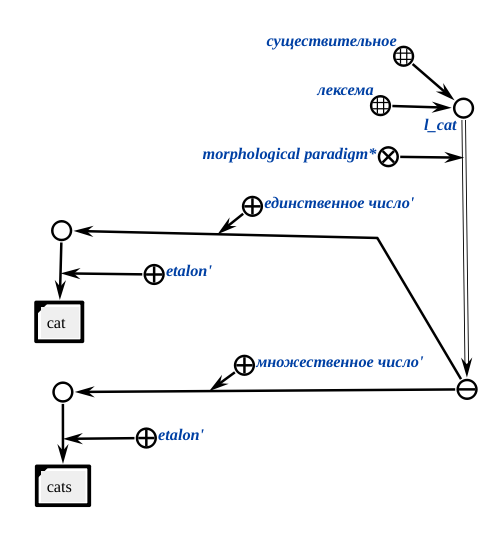
\includegraphics[scale=0.8]{images/part2/chapter_lang/lexeme_example}
    \label{fig:lexeme_example}
\end{figure}

\textbf{\textit{часть речи}} --- \textit{категория}, представляющая собой класс синтаксически эквивалентных \textit{знаков} \textit{естественного языка}.

\begin{SCn}

    \scnheader{часть речи}
    \scnrelto{семейство подмножеств}{лексема}
    \scnhaselement{существительное}
    \scnhaselement{прилагательное}
    \scnhaselement{глагол}
    \scnhaselement{наречие}
    \scnhaselement{предлог}
    \scnhaselement{комплементатор}
    \scnhaselement{вспомогательный глагол}
    \scnhaselement{детерминант}

\end{SCn}

\textbf{\textit{морфологическая парадигма*}} --- \textit{бинарное ориентированное отношение}, связывающее \textit{лексему} и множество ее \textit{словоформ}.

\textbf{\textit{словоформа}} --- \textit{подмножество} \textit{лексемы}, которому принадлежат все вхождения \textit{лексемы} с определенными \textit{грамматическими значениями}.
В рамках нашей \textit{онтологии} словоформа понимается несколько иначе, чем принято в лингвистике, так как все вхождения лексемы в технологии OSTIS являются \textit{файлами}.

При формализации синтаксиса в основном использовались стандартные положения генеративной грамматики (см.~\scncite{Adger2003}, \scncite{Jackendoff1977}, \scncite{Haegeman1994}, \scncite{Carnie2012}).

\textbf{\textit{дистрибуция знака}} –- это подмножество синтаксических правил, в которые входит данный \textit{знак}.

\textbf{\textit{составляющая}} --- элемент множества \textit{C} подмножеств кортежа вхождений лексем \textit{S}, которое содержит в качестве элементов как сам \textit{S}, так и все вхождения лексем в \textit{S}, таким образом, что любые два подмножества, входящие в \textit{C}, либо не пересекаются, либо одно из них включается в другое.

\textbf{\textit{непосредственно составляющая}} ---  есть множество \textit{составляющих} \textit{S}, в которое входят \textit{составляющие} \textit{A} и \textit{B}. В является \textit{непосредственно составляющей} \textit{А} если и только если \textit{В} является подмножеством \textit{А} и нет такой \textit{составляющей} \textit{С}, которая является подмножеством \textit{А} и подмножеством которой является \textit{В}.

\textbf{\textit{составляющими-сестрами*}} считаются \textit{составляющие}, являющиеся \textit{непосредственно составляющими} одной и той же \textit{составляющей}.

Связи между составляющими представлены на~\textit{\nameref{fig:syntactic_example}}.

\begin{figure}[H]
    \centering
    \caption{Рисунок. Иллюстрация связей между составляющими.}
    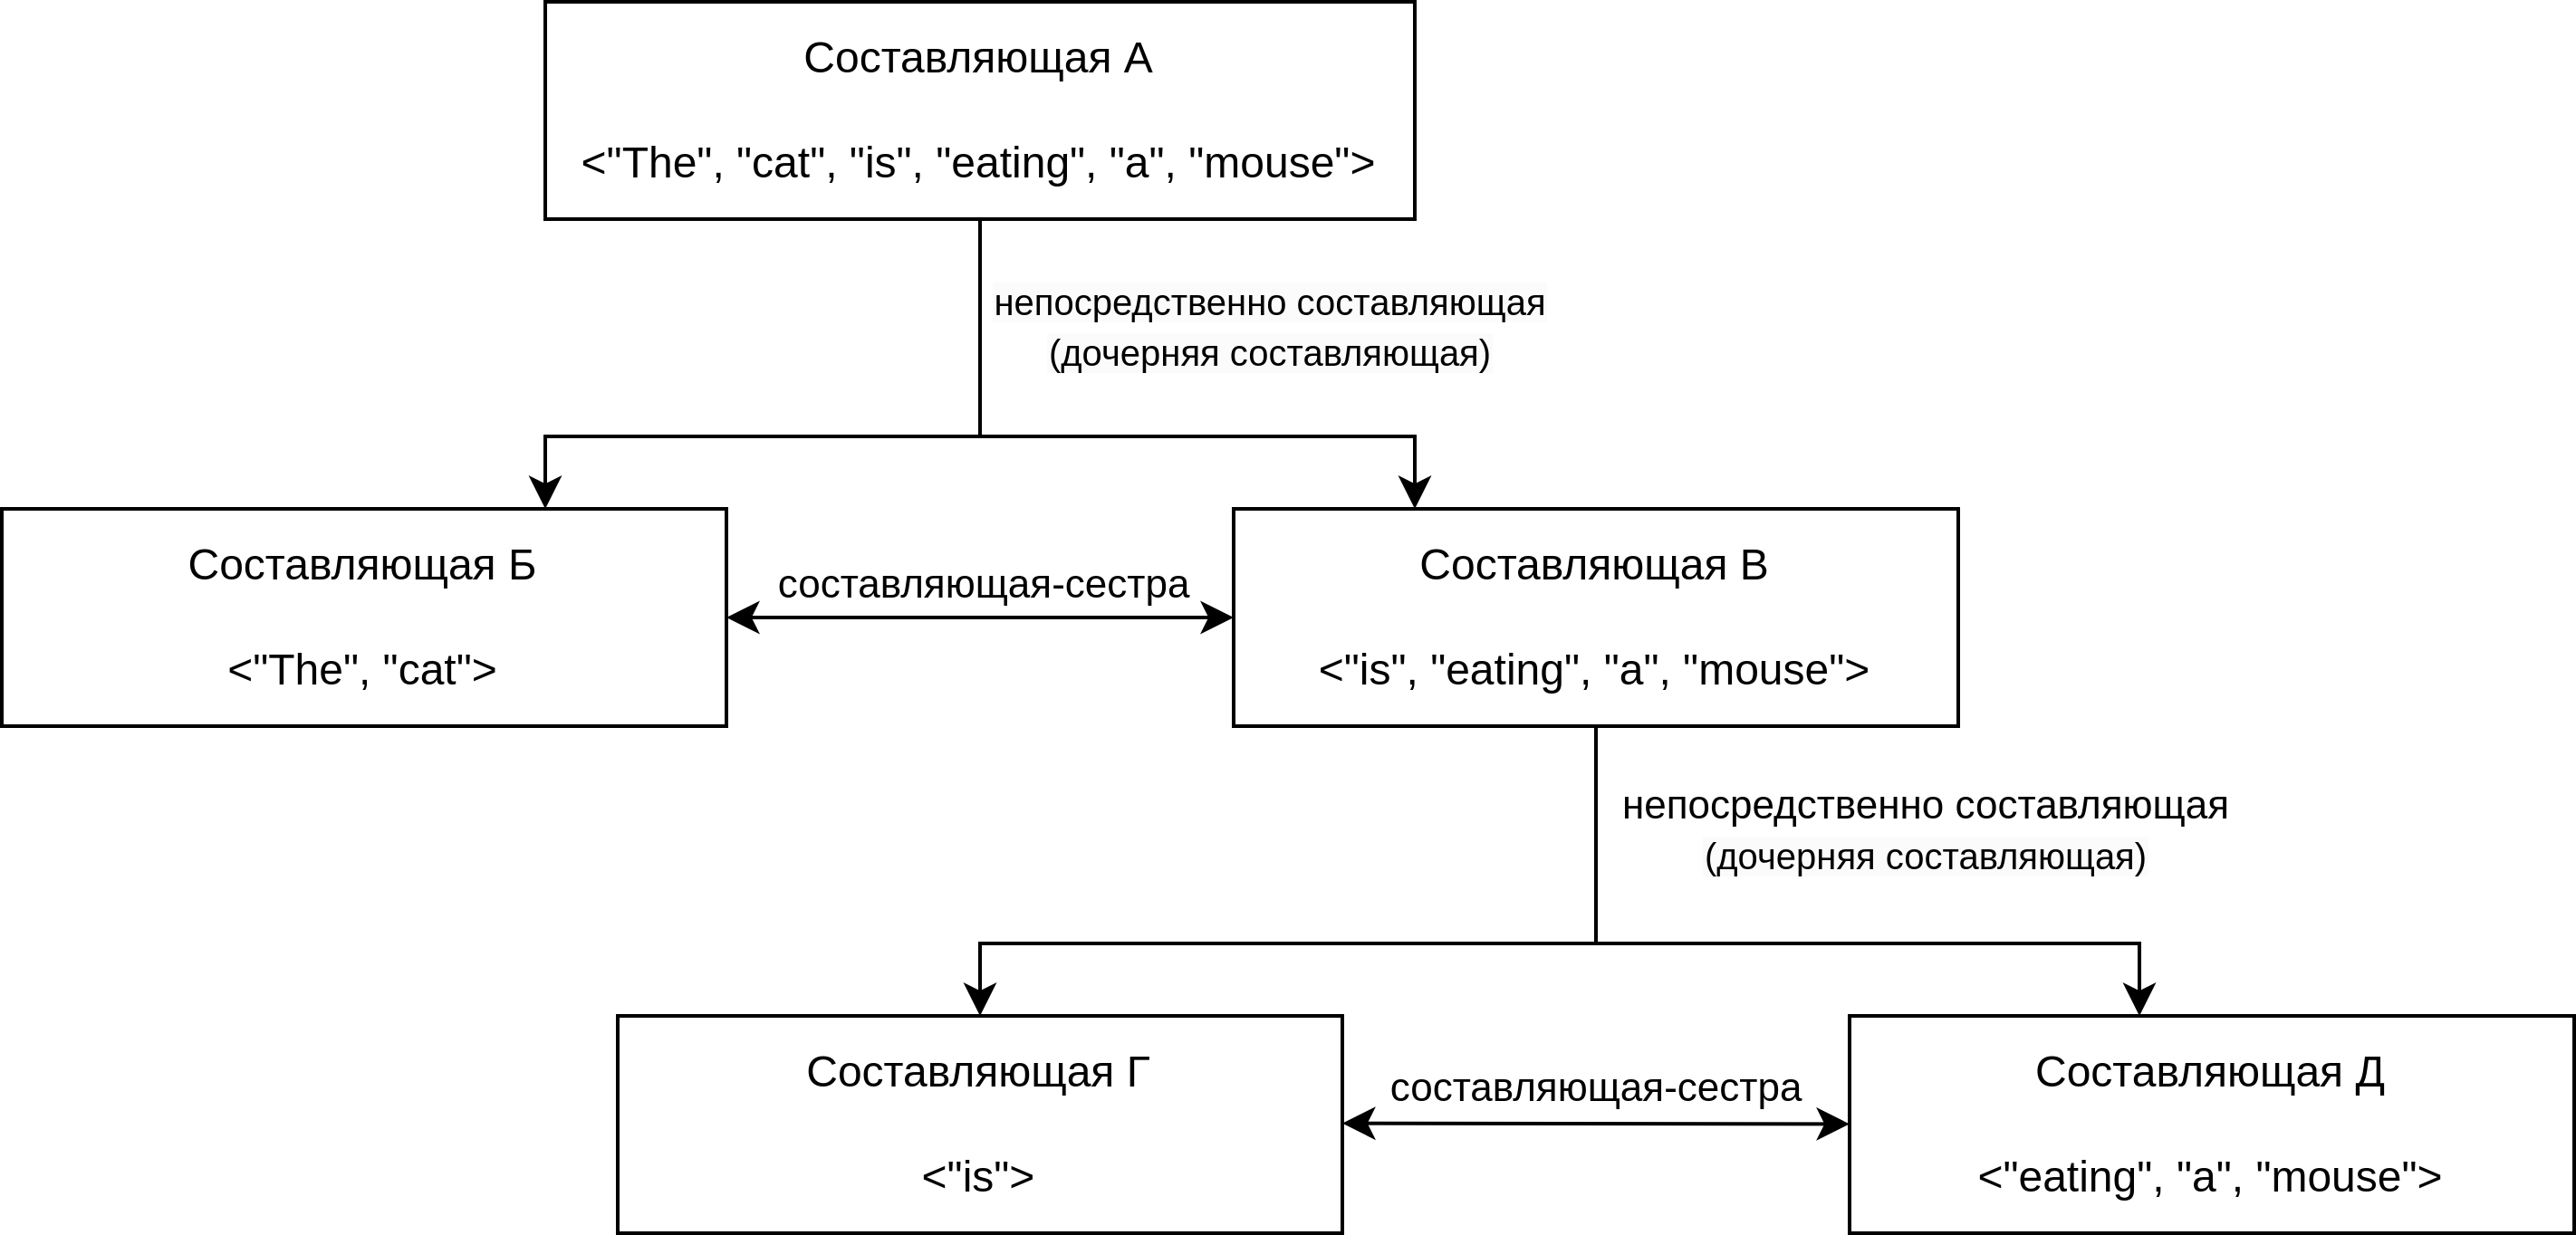
\includegraphics[scale=0.15]{images/part2/chapter_lang/syntactic_example}
    \label{fig:syntactic_example}
\end{figure}

\textbf{\textit{элементарная составляющая}} --- элемент кортежа вхождений \textit{лексем} \textit{L}, являющихся \textit{непосредственно составляющими} множества \textit{составляющих} \textit{C} и не имеющих непосредственно составляющих \textit{составляющих}.

\textbf{\textit{синтаксическая группа}} --- класс \textit{составляющих}, в который входят \textit{составляющие} с вершинами, принадлежащими к одной \textit{части речи}.
\textit{синтаксические группы} представляют собой либо \textit{синглетон} (минимально включают в себя вершину), либо упорядоченную пару, состояющую из \textit{вершины} и другой \textit{синтаксической группы}.

\textbf{\textit{вершина}} --- \textit{составляющая}, \textit{дистрибуция} которой совпадает с \textit{дистрибуцией} всей \textit{синтаксической группы}.

\begin{SCn}

    \scnheader{составляющая}
    \begin{scnrelfromset}{разбиение}
        \scnitem{синтаксическая группа}
        \scnitem{вершина}
    \end{scnrelfromset}

    \scnheader{синтаксическая группа}
    \begin{scnrelfromset}{разбиение}
        \scnitem{именная группа}
        \begin{scnindent}
            \scntext{пояснение}{\textit{Именная группа} --- \textit{синтаксическая группа}, \textit{вершиной} которой является \textit{существительное}.}
        \end{scnindent}
        \scnitem{глагольная группа}
        \begin{scnindent}
            \scntext{пояснение}{\textit{Глагольная группа} --- \textit{синтаксическая группа}, \textit{вершиной} которой является \textit{глагол}.}
        \end{scnindent}
        \scnitem{группа прилагательного}
        \begin{scnindent}
            \scntext{пояснение}{\textit{Группа прилагательного} --- \textit{синтаксическая группа}, \textit{вершиной} которой является \textit{прилагательное}.}
        \end{scnindent}
        \scnitem{наречная группа}
        \begin{scnindent}
            \scntext{пояснение}{\textit{Наречная группа} --- \textit{синтаксическая группа}, \textit{вершиной} которой является \textit{наречие}.}
        \end{scnindent}
        \scnitem{предложная группа}
        \begin{scnindent}
            \scntext{пояснение}{\textit{Предложная группа} --- \textit{синтаксическая группа}, \textit{вершиной} которой является \textit{предлог}.}
        \end{scnindent}
        \scnitem{группа комплементатора}
        \begin{scnindent}
            \scntext{пояснение}{\textit{Группа комплементатора} --- \textit{синтаксическая группа}, \textit{вершиной} которой является \textit{комплементатор}.}
        \end{scnindent}
        \scnitem{временная группа}
        \begin{scnindent}
            \scntext{пояснение}{\textit{Временная группа} --- \textit{синтаксическая группа}, \textit{вершиной} которой является \textit{вспомогательный} либо \textit{модальный глагол}.}
        \end{scnindent}
        \scnitem{группа детерминанта}
        \begin{scnindent}
            \scntext{пояснение}{\textit{Группа детерминанта} --- \textit{синтаксическая группа}, \textit{вершиной} которой является \textit{детерминант}.}
        \end{scnindent}
    \end{scnrelfromset}
    \begin{scnrelfromset}{разбиение}
        \scnitem{максимальная проекция вершины}
            \begin{scnindent}
            \scnidtf{максимальная проекция вершины синтаксической группы}
            \end{scnindent}
        \scnitem{промежуточная проекция вершины}
            \begin{scnindent}
            \scnidtf{промежуточная проекция вершины синтаксической группы}
            \end{scnindent}
    \end{scnrelfromset}

\end{SCn}

При этом для упрощения могут быть введены более узкие классы, являющиеся пересечением приведенных выше, например \textit{максимальная проекция вершины группы детерминанта}.

\begin{SCn}

    \scnheader{максимальная проекция вершины группы детерминанта}
    \begin{scnreltoset}{пересечение}
        \scnitem{группа детерминанта}
        \scnitem{максимальная проекция вершины}
    \end{scnreltoset}

\end{SCn}

Пример синтаксической структуры предложения, записанный с применением введенных выше понятий представлен на~\textit{\nameref{fig:pic_syntactic_tree_part_1}} и~\textit{\nameref{fig:pic_syntactic_tree_part_2}}.

\begin{figure*}[h]
    \caption{SCg-текст. Иллюстрация синтаксической структуры предложения. Первая часть}
    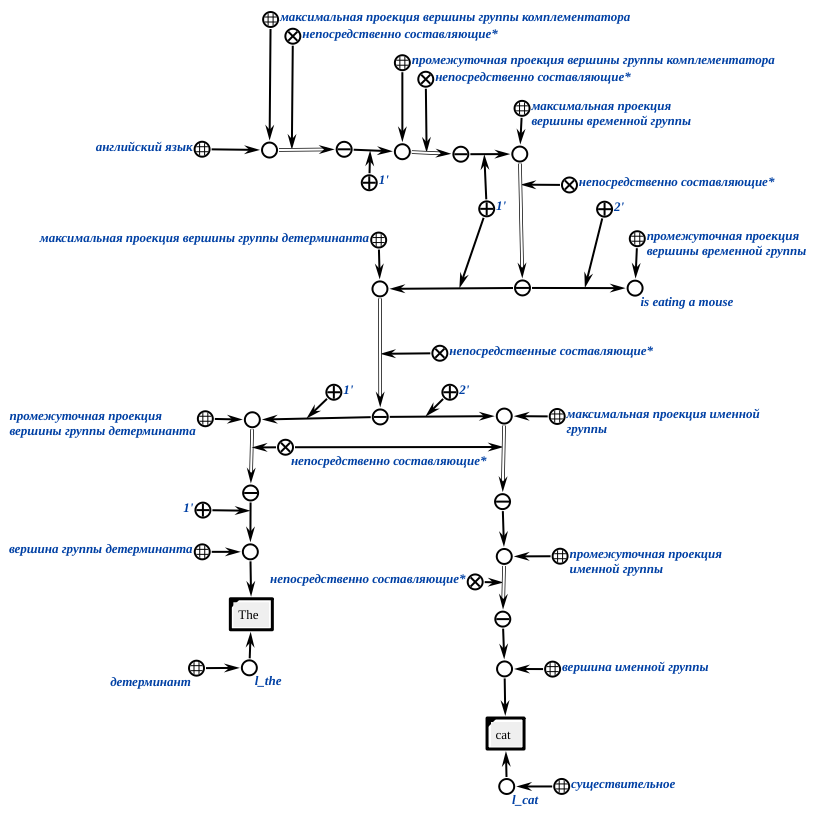
\includegraphics[scale=0.8]{images/part2/chapter_lang/syntactic_structure_part_1}
    \label{fig:pic_syntactic_tree_part_1}
\end{figure*}

\begin{figure*}[h]
    \caption{SCg-текст. Иллюстрация синтаксической структуры предложения. Вторая часть}
    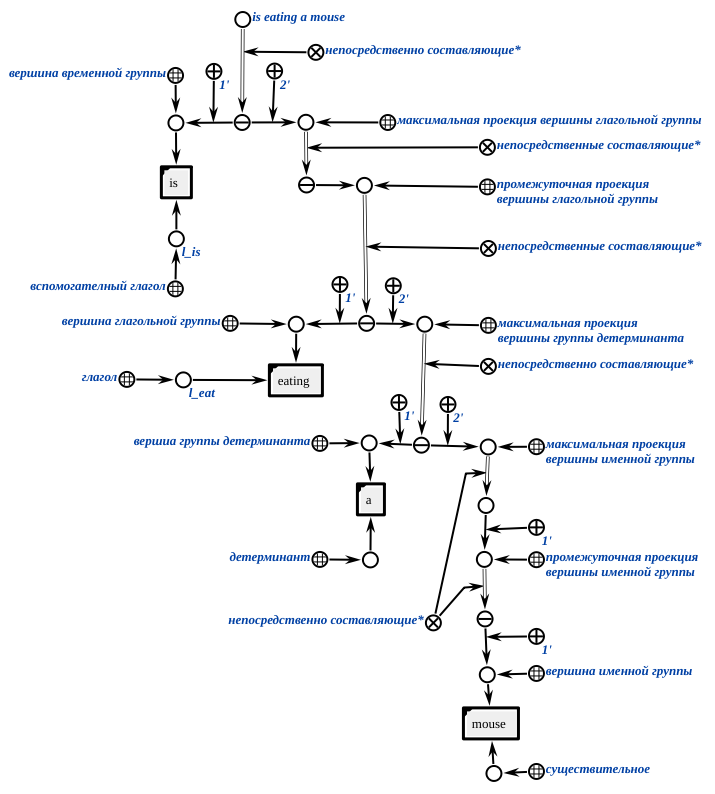
\includegraphics[scale=0.8]{images/part2/chapter_lang/syntactic_structure_part_2}
    \label{fig:pic_syntactic_tree_part_2}
\end{figure*}

Структуры синтаксических групп не являются произвольными --- элементы внутри группы могут граничить только с определенными множествами элементов.
Ниже приводятся возможные структуры синтаксических групп.
В скобках указаны опциональные элементы.

Группа детерминанта:
\begin{textitemize}
    \item \textit{максимальная проекция вершины группы детерминанта} состоит из (\textit{максимальной проекции вершины группы детерминанта}) и \textit{промежуточной проекции вершины группы детерминанта};
    \item \textit{промежуточная проекция вершины группы детерминанта} состоит из \textit{вершины группы детерминанта} (и \textit{максимальной проекции вершины именной группы}).
\end{textitemize}

Именная группа:
\begin{textitemize}
    \item \textit{максимальная проекция вершины именной группы} состоит из (\textit{максимальной проекции вершины группы детерминанта}) и \textit{промежуточной проекции вершины именной группы};
    \item \textit{промежуточная проекция вершины именной группы} состоит из (\textit{максимальной проекции вершины группы прилагательного}) и \textit{промежуточной проекции вершины именной группы} ИЛИ \textit{промежуточной проекции вершины именной группы} (и \textit{максимальной проекции вершины предложной группы});
    \item \textit{промежуточная проекция вершины именной группы} состоит из \textit{вершины именной группы} (и \textit{максимальной проекции вершины предложной группы}).
\end{textitemize}

Глагольная группа:
\begin{textitemize}
    \item \textit{максимальная проекция вершины глагольной группы} состоит из \textit{промежуточная проекция вершины глагольной группы};
    \item \textit{промежуточная проекция вершины глагольной группы} состоит из \textit{промежуточной проекции вершины глагольной группы} (и \textit{максимальной проекции вершины предложной группы}) ИЛИ \textit{промежуточной проекции вершины глагольной группы} (и \textit{максимальной проекция вершины наречной группы});
    \item \textit{промежуточная проекция вершины глагольной группы} состоит из \textit{вершины глагольной группы} (и \textit{максимальной проекции вершины именной группы}).
\end{textitemize}

Наречная группа:
\begin{textitemize}
    \item \textit{максимальная проекция вершины наречной группы} состоит из \textit{промежуточной проекции вершины наречной группы};
    \item \textit{промежуточная проекция вершины наречной группы} состоит из (\textit{максимальной проекции вершины наречной группы}) и \textit{промежуточной проекции вершины наречной группы};
    \item \textit{промежуточная проекция вершины наречной группы} состоит из \textit{вершины наречной группы} (и \textit{максимальной проекции вершины предложной группы}).
\end{textitemize}

Группа прилагательного:
\begin{textitemize}
    \item \textit{максимальная проекция вершины группы прилагательного} состоит из \textit{промежуточной проекции вершины группы прилагательного};
    \item \textit{промежуточная проекция вершины группы прилагательного} состоит из (\textit{максимальной проекции вершины наречной группы}) и \textit{промежуточной проекции вершины группы прилагательного};
    \item \textit{промежуточная проекция вершины группы прилагательного} состоит из \textit{вершины группы прилагательного} (и \textit{максимальной проекцим вершины предложной группы}).
\end{textitemize}

Предложная группа:
\begin{textitemize}
    \item \textit{максимальная проекция вершины предложной группы} состоит из \textit{промежуточной проекции вершины предложной группы};
    \item \textit{промежуточная проекция вершины предложной группы} состоит из \textit{промежуточной проекции вершины предложной группы} (и \textit{максимальной проекции вершины предложной группы}) ИЛИ (\textit{максимальной проекции вершины наречной группы}) и \textit{промежуточной проекции вершины предложной группы};
    \item \textit{промежуточная проекция вершины предложной группы} состоит из \textit{вершины предложной группы} (и \textit{максимальной проекции вершины именной группы}).
\end{textitemize}

Временная группа:
\begin{textitemize}
    \item \textit{максимальная проекция вершины временной группы} состоит из (\textit{максимальной проекции вершины группы детерминанта}) и \textit{промежуточной проекции вершины временной группы};
    \item \textit{промежуточная проекция вершины временной группы} состоит из \textit{вершины временной группы} (и \textit{максимальной проекции вершины глагольной группы}).
\end{textitemize}

Группа комплементатора:
\begin{textitemize}
    \item \textit{максимальная проекция вершины группы комплементатора} состоит из (\textit{максимальной проекции вершины некоторой синтаксической группы}) и \textit{промежуточной проекции вершины группы комплементатора};
    \item \textit{промежуточная проекция вершины группы комплементатора} состоит из \textit{вершины группы комплементатора} \textit{и максимальной проекции вершины временной группы}.
\end{textitemize}

В формальном виде данные правила можно представить следующим образом (см.~\textit{\nameref{fig:pic_tree_structure_rule}}).

\begin{figure*}[h]
    \caption{SCg-текст. Иллюстрация правила структуры синтаксической группы}
    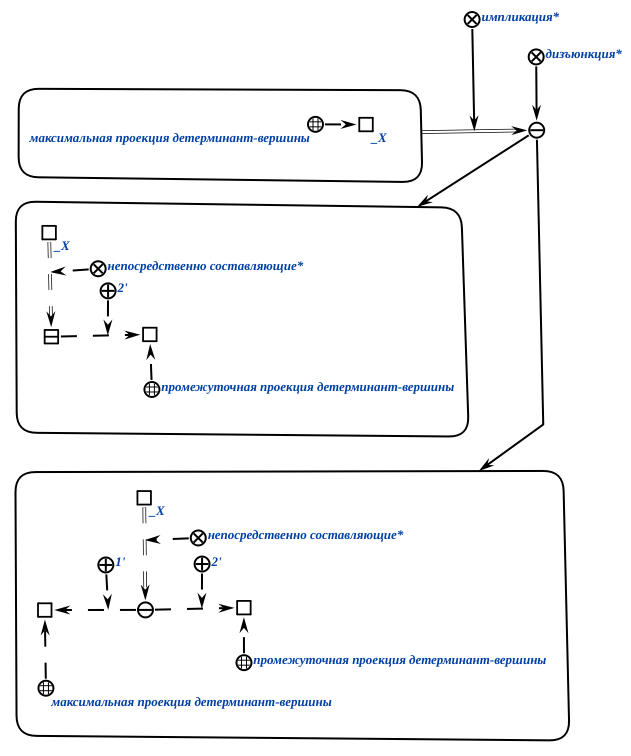
\includegraphics[scale=0.8]{images/part2/chapter_lang/tree_structure_rule}
    \label{fig:pic_tree_structure_rule}
\end{figure*}

\textbf{\textit{комплемент}} --- \textit{синтаксическая группа}, являющаяся сестрой вершины.

\textbf{\textit{адъюнкт}} --- \textit{синтаксическая группа}, являющаяся дочерью (\textit{непосредственно составляющей}) промежуточной проекции и сестрой промежуточной проекции вершины той же \textit{синтаксической группы}.

\textbf{\textit{спецификатор}} --- \textit{синтаксическая группа}, являющейся дочерью максимальной проекции и сестрой промежуточной проекции.

Приведенные выше правила структуры синтаксических групп можно обобщить и свести к трем более абстрактным.

Правило спецификатора: \textit{максимальная проекция вершины синтаксической группы} \textit{XP} состоит из (\textit{максимальной проекции вершины} \textit{YP}) \textit{промежуточной проекции вершины синтаксической группы} \textit{X'}

В формализованном виде данное правило представлено на~\textit{\nameref{fig:specifier_rule}}.

\begin{figure*}[h]
    \caption{SCg-текст. Правило спецификатора}
    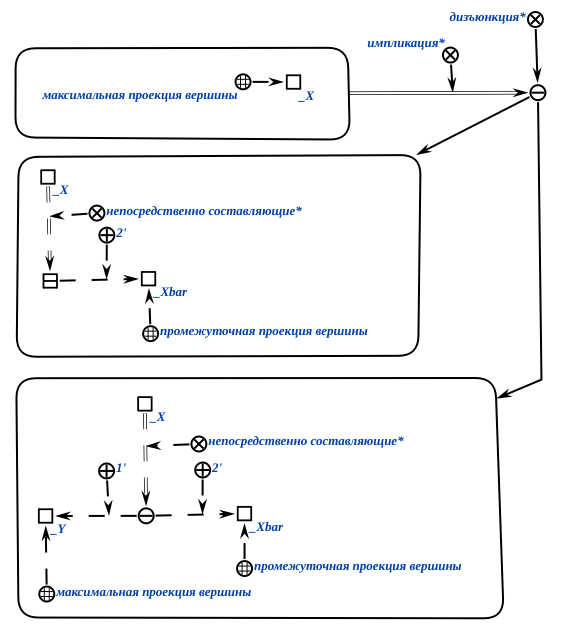
\includegraphics[scale=0.8]{images/part2/chapter_lang/specifier_rule}
    \label{fig:specifier_rule}
\end{figure*}

Правило адъюнкта: \textit{промежуточная проекция вершины синтаксической группы} \textit{X'} состоит из \textit{промежуточной проекции вершины синтаксической группы} \textit{$\bm{X'_1}$} (и \textit{максимальной проекции вершины синтаксической группы} \textit{ZP}) ИЛИ из (\textit{максимальной проекции вершины синтаксической группы} \textit{ZP}) и \textit{промежуточной проекции вершины синтаксической группы} \textit{X'}.

%todo какое-то пояснение

В формализованном виде данное правило представлено на~\textit{\nameref{fig:adjunct_rule}}.

\begin{figure*}[h]
    \caption{SCg-текст. Правило адъюнкта}
    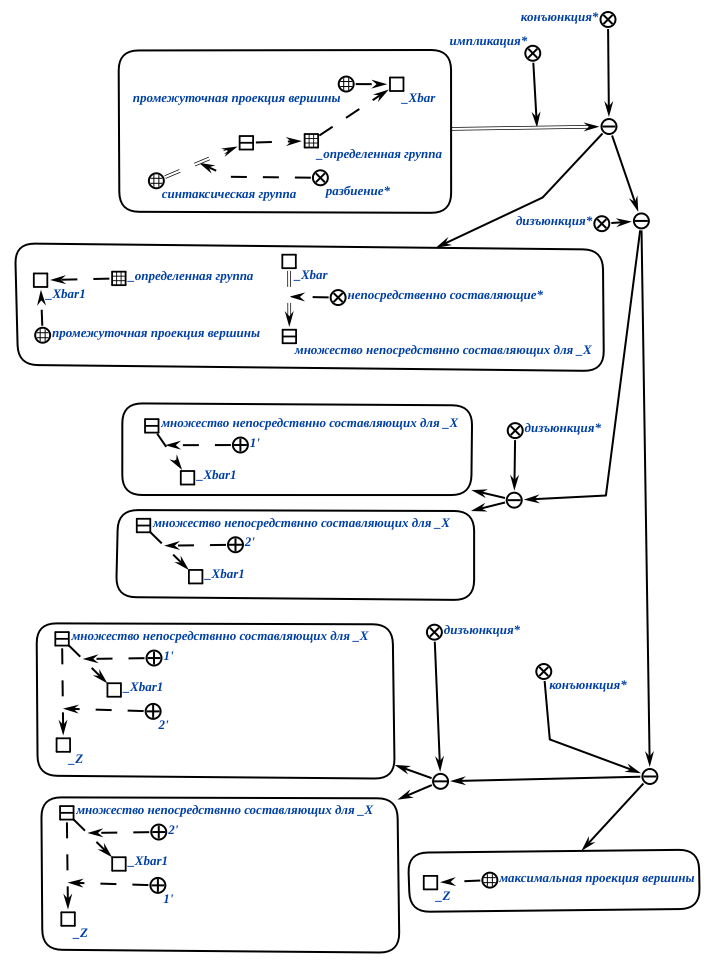
\includegraphics[scale=0.8]{images/part2/chapter_lang/adjunct_rule}
    \label{fig:adjunct_rule}
\end{figure*}

Правило комплемента: \textit{промежуточная проекция вершины синтаксической группы}  \textit{X'} состоит из \textit{вершины} \textit{X} (и \textit{максимальной проекции вершины синтаксической группы} \textit{WP}).

В формализованном виде данное правило представлено на~\textit{\nameref{fig:complement_rule}}.

\begin{figure*}[h]
    \caption{SCg-текст. Правило комплемента}
    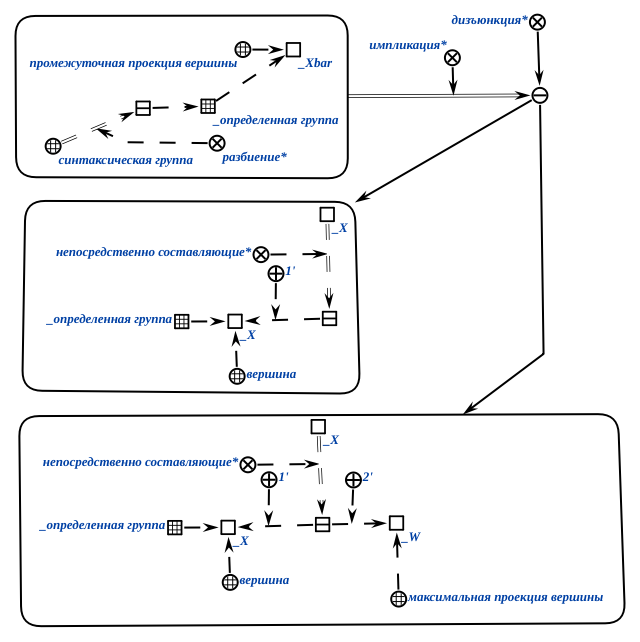
\includegraphics[scale=0.8]{images/part2/chapter_lang/complement_rule}
    \label{fig:complement_rule}
\end{figure*}


Формальное представление данных правил аналогично приведенному на~\textit{\nameref{fig:pic_tree_structure_rule}}.

\section{Формализация денотационной семантики естественных языков}
\label{section_natural_language_denotational_semantics_formalization}

Формализацией \textit{денотационной семантики} \textit{естественного языка} мы будем считать множество общих правил перехода от \textit{синтаксиса информационных конструкций} \textit{естественных языков} к \textit{смысловому представлению информации}, содержащейся в исходной \textit{информационной конструкции}.

\textit{денотационная семантика} \textit{языка} специфицирует интерпретацию элементов \textit{синтаксиса} данного \textit{языка} и представляет собой множество формул, описывающих то, каким образом \textit{информационным конструкциям} \textit{языка} ставятся в соответствие обозначаемые ими сущности и конфигурации отношений между этими сущностями.

\textit{денотационная семантика} \textit{естественных языков} должна обладать свойством композициональности --- то есть интерпретация всего высказывания должна выводиться из интерпретации отдельных его частей.
Таким образом, необходимо предоставить формальное описание интерпретации элементов \textit{синтаксиса} \textit{естественного языка}, представленных в предыдущем разделе, а также описание правил совмещения интерпретации отдельных элементов для получения \textit{смысла} всего высказывания.

В данной главе мы предлагаем вариант формализации \textit{денотационной семантики} \textit{естественных языков} в рамках \textit{Технологии OSTIS}, для составления которой использовались стандартные положения формальной семантики (см.~\scncite{Heim1998}, \scncite{Winter2016}, \scncite{Portner2008}).

Рассмотрим примеры правил, реализующих \textit{денотационную семантику} \textit{языка}.
Приведенные ниже правила должны применяться последовательно и позволяют получить \textit{смысл} текста \textit{естественного языка} по его синтаксической структуре, "поднимаясь"{} по дереву \textit{составляющих} от \textit{вершин} к \textit{максимальным проекциям}.

На~\textit{\nameref{fig:d_sem_1}} приведено правило, по которому происходит интерпретация вершин \textit{именной группы} и \textit{группы прилагательного}.
Смыслом таких вершин является класс, например: \textit{прилагательному} "черный"{} соответствует множество черных объектов, а \textit{существительному} "кот"{} --- множество котов.

\begin{figure}[h]
    \caption{SCg-текст. Правило интерпретации вершины группы прилагательного и вершины именной группы}
    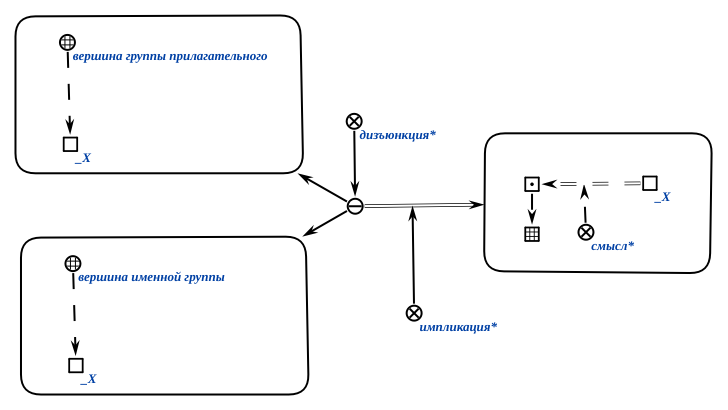
\includegraphics[scale=0.8]{images/part2/chapter_lang/d_sem_1}
    \label{fig:d_sem_1}
\end{figure}

На~\textit{\nameref{fig:d_sem_2}} приведено правило, по которому происходит интерпретация \textit{именной группы}, максимальная проекция которой включается в себя также группу прилагательного.
Как говорилось выше, для применения данного правила необходимо предварительное применение правила, представленного на~\textit{\nameref{fig:d_sem_1}}.

Смыслом таких конструкций является класс, являющийся результатом \textit{пересечения} классов, полученных в результате интерпретации \textit{вершин} \textit{групп прилагательного} и \textit{именной группы} по отдельности.
Например: \textit{черный кот} --- множество черных котов, пересечение множества котов и черных объектов. %ну все, теперь включаю мою кошку в соавторы

\begin{figure*}[h]
    \caption{SCg-текст. Правило интерпретации максимальной проекции вершины именной группы}
    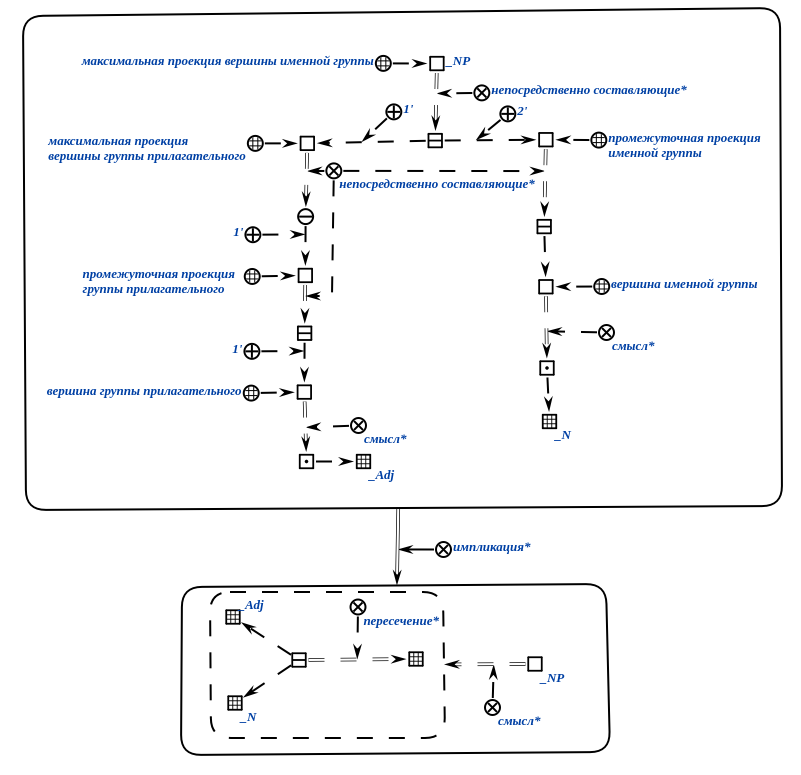
\includegraphics[scale=0.8]{images/part2/chapter_lang/d_sem_2}
    \label{fig:d_sem_2}
\end{figure*}
%тут мы комбинируем смыслы прилагательного и существительного, которые входят в одну именную группу

На~\textit{\nameref{fig:d_sem_3}} приведено правило, по которому происходит интерпретация \textit{глагольной группы}.
Необходимость включения в посылку правила всей ветки глагольной группы объясняется ее необходимостью для определения типа \textit{глагола} --- данное правило предназначено для интерпретации непереходных \textit{глаголов}.
\textit{смыслом} такой конструкции является класс \textit{действий}.

\begin{figure*}[h]
    \caption{SCg-текст. Правило интерпретации максимальной проекции вершины глагольной группы, содержащей непереходный глагол}
    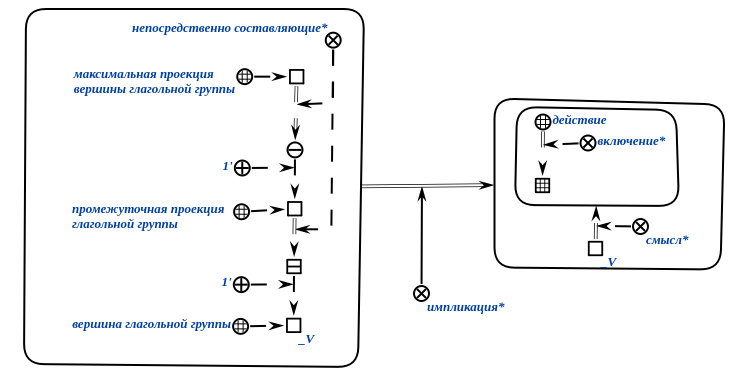
\includegraphics[scale=0.8]{images/part2/chapter_lang/d_sem_3}
    \label{fig:d_sem_3}
\end{figure*}
%тут мы задаем интерпретацию всей глагольной группы (макс проекции) только для непереходных глаголов. написать, что смотрим по всей структуре группы целиком, потому что для того, чтобы отличить непереходный от переходного нам нужна вся ветка глагольной группы в дереве целиком

На~\textit{\nameref{d_sem_4}} приведено правило, по которому происходит интерпретация \textit{группы детерминанта} с неопределенным артиклем.
Смыслом такой конструкции является существование элемента класса, являющегося \textit{смыслом} входящей в состав данной \textit{группы детерминанта} \textit{именной группы}.

\begin{figure*}[h]
    \caption{SCg-текст. Правило интерпретации максимальной проекции вершины группы детерминанта}
    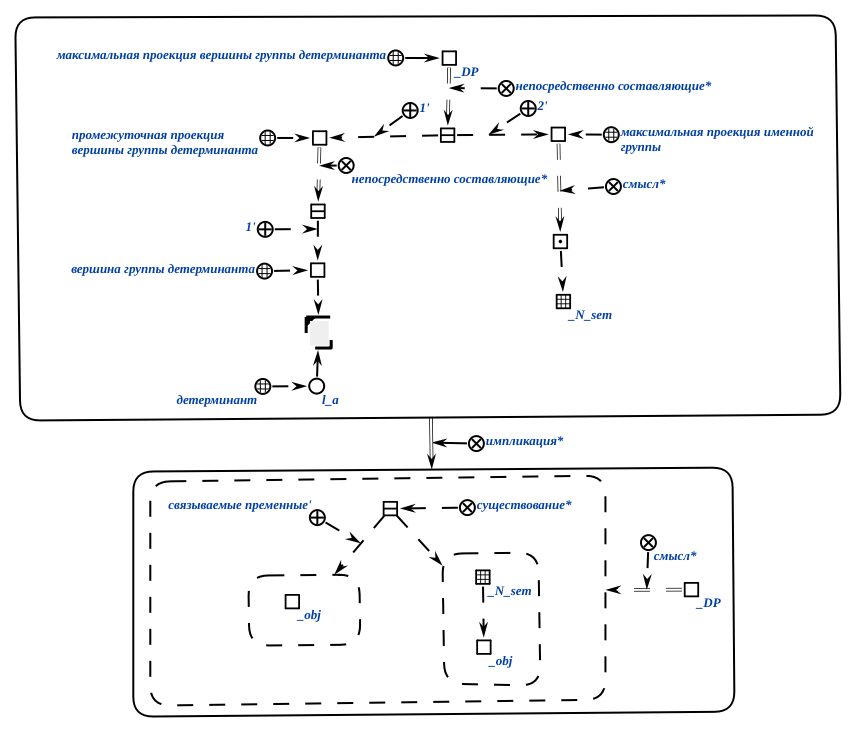
\includegraphics[scale=0.8]{images/part2/chapter_lang/d_sem_4}
    \label{d_sem_4}
\end{figure*}
%тут задается интерпретация сочетания именной группы с артиклем (в данном случае неопределенным)

На~\textit{\nameref{fig:d_sem_5}} приведено правило, по которому происходит интерпретация \textit{промежуточной проекции вершины временной группы}, состоящей из вспомогательного \textit{глагола} и полнозначного глагола.
Вспомогательный \textit{глагол} в данном случае задет класс действий по времени (является ли оно запланированным, выполняемым, уже выполненным и так далее).

\begin{figure*}[h]
    \caption{SCg-текст. Правило интерпретации промежуточной проекции вершины временной группы}
    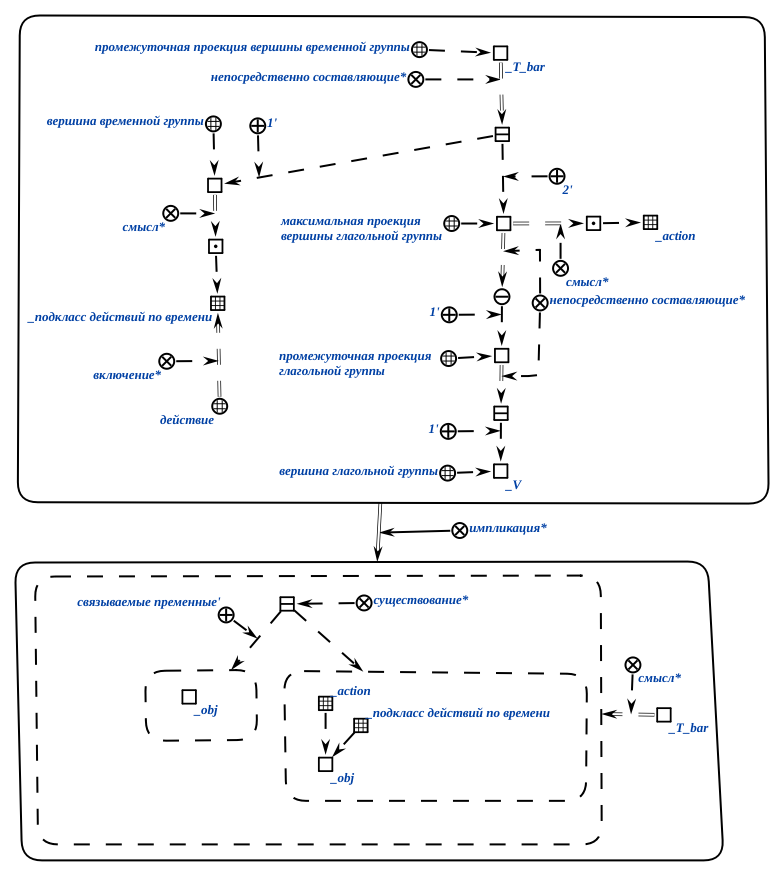
\includegraphics[scale=0.8]{images/part2/chapter_lang/d_sem_5}
    \label{fig:d_sem_5}
\end{figure*}
%тут задаем интерпретацию сочетания вспомогательного глагола и основного глагола. вспомогательный у нас соответствует классу действий по времени

На~\textit{\nameref{fig:d_sem_6}} приведено правило, по которому происходит интерпретация \textit{максимальной проекции вершины временной группы} на основе полученного на предыдущем шаге \textit{смысла} \textit{промежуточной проекции вершины временной группы} и \textit{смысла} \textit{максимальной проекции группы детерминанта}.

\begin{figure*}[h]
    \caption{SCg-текст. Правило интерпретации максимальной проекции вершины временной группы}
    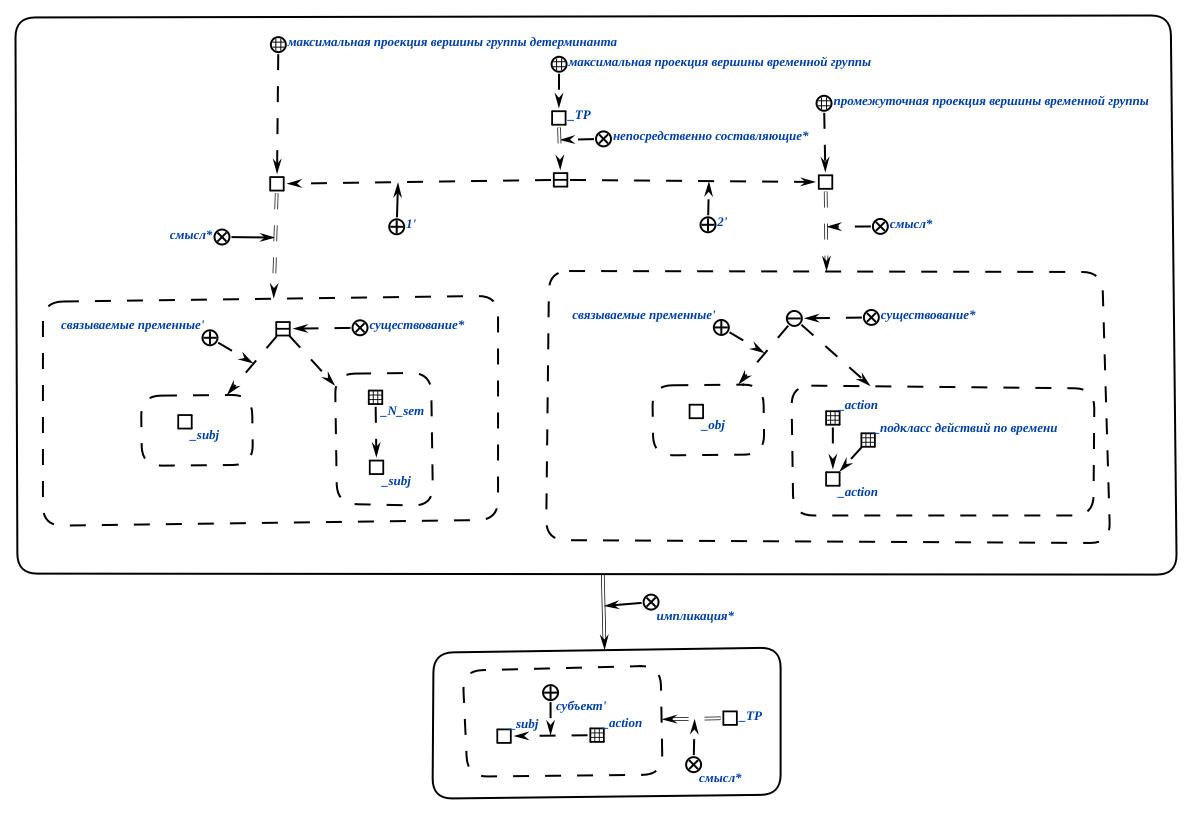
\includegraphics[scale=0.8]{images/part2/chapter_lang/d_sem_6}
    \label{fig:d_sem_6}
\end{figure*}
%тут задаем интерпретацию для аргументной структуры непереходного глагола (сочетания подлежащего с непереходным глаголом)

На~\textit{\nameref{fig:d_sem_7}} приведено правило, по которому происходит интерпретация \textit{максимальной проекции вершины группы комплементатора} на основе полученных на предыдущих шагах \textit{смыслов} более частных конструкций.
Данным правилом задается интерпретация предложения с переходным \textit{глаголом}.

\begin{figure*}[h]
    \caption{SCg-текст. Правило интерпретации предложения с переходным глаголом}
    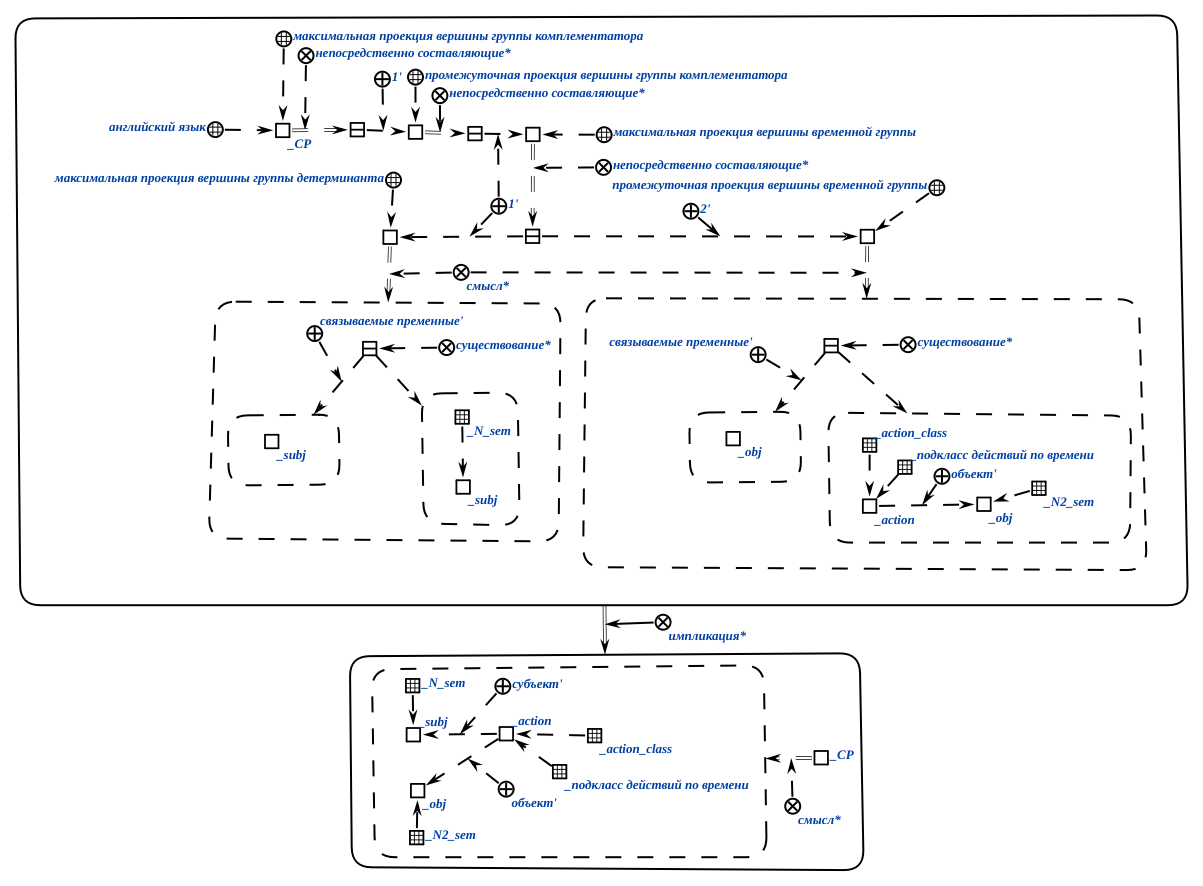
\includegraphics[scale=0.8]{images/part2/chapter_lang/d_sem_7}
    \label{fig:d_sem_7}
\end{figure*}
%тут задаем интерпретацию аргументной структуры переходного глагола (сочетания переходного глагола с его аргументами --- подлажещим и дополнением)

%%%%%%%%%%%%%%%%%%%%%%%%% referenc.tex %%%%%%%%%%%%%%%%%%%%%%%%%%%%%%
% sample references
% %
% Use this file as a template for your own input.
%
%%%%%%%%%%%%%%%%%%%%%%%% Springer-Verlag %%%%%%%%%%%%%%%%%%%%%%%%%%
%
% BibTeX users please use
% \bibliographystyle{}
% \bibliography{}
%
\biblstarthook{In view of the parallel print and (chapter-wise) online publication of your book at \url{www.springerlink.com} it has been decided that -- as a genreral rule --  references should be sorted chapter-wise and placed at the end of the individual chapters. However, upon agreement with your contact at Springer you may list your references in a single seperate chapter at the end of your book. Deactivate the class option \texttt{sectrefs} and the \texttt{thebibliography} environment will be put out as a chapter of its own.\\\indent
References may be \textit{cited} in the text either by number (preferred) or by author/year.\footnote{Make sure that all references from the list are cited in the text. Those not cited should be moved to a separate \textit{Further Reading} section or chapter.} If the citatiion in the text is numbered, the reference list should be arranged in ascending order. If the citation in the text is author/year, the reference list should be \textit{sorted} alphabetically and if there are several works by the same author, the following order should be used:
\begin{enumerate}
\item all works by the author alone, ordered chronologically by year of publication
\item all works by the author with a coauthor, ordered alphabetically by coauthor
\item all works by the author with several coauthors, ordered chronologically by year of publication.
\end{enumerate}
The \textit{styling} of references\footnote{Always use the standard abbreviation of a journal's name according to the ISSN \textit{List of Title Word Abbreviations}, see \url{http://www.issn.org/en/node/344}} depends on the subject of your book:
\begin{itemize}
\item The \textit{two} recommended styles for references in books on \textit{mathematical, physical, statistical and computer sciences} are depicted in ~\cite{science-contrib, science-online, science-mono, science-journal, science-DOI} and ~\cite{phys-online, phys-mono, phys-journal, phys-DOI, phys-contrib}.
\item Examples of the most commonly used reference style in books on \textit{Psychology, Social Sciences} are~\cite{psysoc-mono, psysoc-online,psysoc-journal, psysoc-contrib, psysoc-DOI}.
\item Examples for references in books on \textit{Humanities, Linguistics, Philosophy} are~\cite{humlinphil-journal, humlinphil-contrib, humlinphil-mono, humlinphil-online, humlinphil-DOI}.
\item Examples of the basic Springer style used in publications on a wide range of subjects such as \textit{Computer Science, Economics, Engineering, Geosciences, Life Sciences, Medicine, Biomedicine} are ~\cite{basic-contrib, basic-online, basic-journal, basic-DOI, basic-mono}. 
\end{itemize}
}

\begin{thebibliography}{99.}%
% and use \bibitem to create references.
%
% Use the following syntax and markup for your references if 
% the subject of your book is from the field 
% "Mathematics, Physics, Statistics, Computer Science"
%
% Contribution 
\bibitem{science-contrib} Broy, M.: Software engineering --- from auxiliary to key technologies. In: Broy, M., Dener, E. (eds.) Software Pioneers, pp. 10-13. Springer, Heidelberg (2002)
%
% Online Document
\bibitem{science-online} Dod, J.: Effective substances. In: The Dictionary of Substances and Their Effects. Royal Society of Chemistry (1999) Available via DIALOG. \\
\url{http://www.rsc.org/dose/title of subordinate document. Cited 15 Jan 1999}
%
% Monograph
\bibitem{science-mono} Geddes, K.O., Czapor, S.R., Labahn, G.: Algorithms for Computer Algebra. Kluwer, Boston (1992) 
%
% Journal article
\bibitem{science-journal} Hamburger, C.: Quasimonotonicity, regularity and duality for nonlinear systems of partial differential equations. Ann. Mat. Pura. Appl. \textbf{169}, 321--354 (1995)
%
% Journal article by DOI
\bibitem{science-DOI} Slifka, M.K., Whitton, J.L.: Clinical implications of dysregulated cytokine production. J. Mol. Med. (2000) doi: 10.1007/s001090000086 
%
\bigskip

% Use the following (APS) syntax and markup for your references if 
% the subject of your book is from the field 
% "Mathematics, Physics, Statistics, Computer Science"
%
% Online Document
\bibitem{phys-online} J. Dod, in \textit{The Dictionary of Substances and Their Effects}, Royal Society of Chemistry. (Available via DIALOG, 1999), 
\url{http://www.rsc.org/dose/title of subordinate document. Cited 15 Jan 1999}
%
% Monograph
\bibitem{phys-mono} H. Ibach, H. L\"uth, \textit{Solid-State Physics}, 2nd edn. (Springer, New York, 1996), pp. 45-56 
%
% Journal article
\bibitem{phys-journal} S. Preuss, A. Demchuk Jr., M. Stuke, Appl. Phys. A \textbf{61}
%
% Journal article by DOI
\bibitem{phys-DOI} M.K. Slifka, J.L. Whitton, J. Mol. Med., doi: 10.1007/s001090000086
%
% Contribution 
\bibitem{phys-contrib} S.E. Smith, in \textit{Neuromuscular Junction}, ed. by E. Zaimis. Handbook of Experimental Pharmacology, vol 42 (Springer, Heidelberg, 1976), p. 593
%
\bigskip
%
% Use the following syntax and markup for your references if 
% the subject of your book is from the field 
% "Psychology, Social Sciences"
%
%
% Monograph
\bibitem{psysoc-mono} Calfee, R.~C., \& Valencia, R.~R. (1991). \textit{APA guide to preparing manuscripts for journal publication.} Washington, DC: American Psychological Association.
%
% Online Document
\bibitem{psysoc-online} Dod, J. (1999). Effective substances. In: The dictionary of substances and their effects. Royal Society of Chemistry. Available via DIALOG. \\
\url{http://www.rsc.org/dose/Effective substances.} Cited 15 Jan 1999.
%
% Journal article
\bibitem{psysoc-journal} Harris, M., Karper, E., Stacks, G., Hoffman, D., DeNiro, R., Cruz, P., et al. (2001). Writing labs and the Hollywood connection. \textit{J Film} Writing, 44(3), 213--245.
%
% Contribution 
\bibitem{psysoc-contrib} O'Neil, J.~M., \& Egan, J. (1992). Men's and women's gender role journeys: Metaphor for healing, transition, and transformation. In B.~R. Wainrig (Ed.), \textit{Gender issues across the life cycle} (pp. 107--123). New York: Springer.
%
% Journal article by DOI
\bibitem{psysoc-DOI}Kreger, M., Brindis, C.D., Manuel, D.M., Sassoubre, L. (2007). Lessons learned in systems change initiatives: benchmarks and indicators. \textit{American Journal of Community Psychology}, doi: 10.1007/s10464-007-9108-14.
%
%
% Use the following syntax and markup for your references if 
% the subject of your book is from the field 
% "Humanities, Linguistics, Philosophy"
%
\bigskip
%
% Journal article
\bibitem{humlinphil-journal} Alber John, Daniel C. O'Connell, and Sabine Kowal. 2002. Personal perspective in TV interviews. \textit{Pragmatics} 12:257--271
%
% Contribution 
\bibitem{humlinphil-contrib} Cameron, Deborah. 1997. Theoretical debates in feminist linguistics: Questions of sex and gender. In \textit{Gender and discourse}, ed. Ruth Wodak, 99--119. London: Sage Publications.
%
% Monograph
\bibitem{humlinphil-mono} Cameron, Deborah. 1985. \textit{Feminism and linguistic theory.} New York: St. Martin's Press.
%
% Online Document
\bibitem{humlinphil-online} Dod, Jake. 1999. Effective substances. In: The dictionary of substances and their effects. Royal Society of Chemistry. Available via DIALOG. \\
http://www.rsc.org/dose/title of subordinate document. Cited 15 Jan 1999
%
% Journal article by DOI
\bibitem{humlinphil-DOI} Suleiman, Camelia, Daniel C. O'Connell, and Sabine Kowal. 2002. `If you and I, if we, in this later day, lose that sacred fire...': Perspective in political interviews. \textit{Journal of Psycholinguistic Research}. doi: 10.1023/A:1015592129296.
%
%
%
\bigskip
%
%
% Use the following syntax and markup for your references if 
% the subject of your book is from the field 
% "Computer Science, Economics, Engineering, Geosciences, Life Sciences"
%
%
% Contribution 
\bibitem{basic-contrib} Brown B, Aaron M (2001) The politics of nature. In: Smith J (ed) The rise of modern genomics, 3rd edn. Wiley, New York 
%
% Online Document
\bibitem{basic-online} Dod J (1999) Effective Substances. In: The dictionary of substances and their effects. Royal Society of Chemistry. Available via DIALOG. \\
\url{http://www.rsc.org/dose/title of subordinate document. Cited 15 Jan 1999}
%
% Journal article by DOI
\bibitem{basic-DOI} Slifka MK, Whitton JL (2000) Clinical implications of dysregulated cytokine production. J Mol Med, doi: 10.1007/s001090000086
%
% Journal article
\bibitem{basic-journal} Smith J, Jones M Jr, Houghton L et al (1999) Future of health insurance. N Engl J Med 965:325--329
%
% Monograph
\bibitem{basic-mono} South J, Blass B (2001) The future of modern genomics. Blackwell, London 
%
\end{thebibliography}
